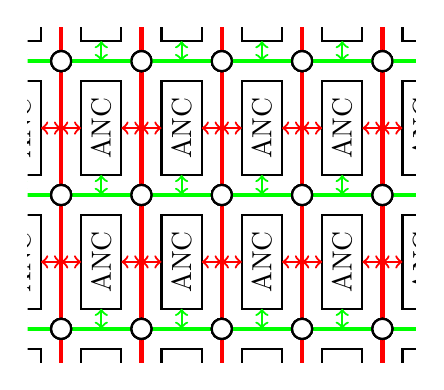
\begin{tikzpicture}[thick,scale=0.17]
	
	\def\xsize{3}
	\def\ysize{7}
	
	\def\w{4}
	\def\h{2}
	
	\def\sp{3}
	\def\swsize{0.5}
	
	\def\clipextra{1}
	
	\pgfmathtruncatemacro{\xsizee}{\xsize+\sp}
	\pgfmathtruncatemacro{\ysizee}{\ysize+\sp}
	
	\clip (-1*\sp - \clipextra, -1*\sp - \clipextra)
	      rectangle ++({\w*(\xsize+\sp) + \sp + 2*\clipextra}, {\h*(\ysize+\sp) + \sp + 2*\clipextra});
	
	% The ANCs in a chip
	\foreach \x in {-1,...,\w}{
		\foreach \y in {-1,...,\h}{
			% The ANC and its label
			\draw (\x*\xsizee,\y*\ysizee) rectangle ++(\xsize, \ysize);
			\node at (\x*\xsizee + 0.5*\xsize,\y*\ysizee + 0.5*\ysize)
			      [rotate=90]
			      {ANC}
			      ;
			% Links to vertical wires
			\draw [<->,red] (\x*\xsizee,0.5*\ysize+\y*\ysizee) -- ++(-0.5*\sp,0);
			\draw [<->,red] (\x*\xsizee+\xsize,0.5*\ysize+\y*\ysizee) -- ++(0.5*\sp,0);
			% Link to horizontal wires
			\draw [<->,green] (0.5*\xsize+\x*\xsizee,\y*\ysizee) -- ++(0,-0.5*\sp);
		}
	}
	
	% The wires
	\foreach \x in {-1,...,\w}{
		\draw [ultra thick,red] (\x*\xsizee - 0.5*\sp, -1*\ysizee) -- ++(0, 2*\h*\ysizee);
	}
	\foreach \y in {-1,...,\h}{
		\draw [ultra thick,green] (-1*\xsizee,\y*\ysizee - 0.5*\sp) -- ++(2*\w*\xsizee, 0);
	
	% The crossbars
	\foreach \x in {-1,...,\w}{
		\foreach \y in {-1,...,\h}{
			\coordinate (corner) at
			            (\x*\xsizee - 0.5*\sp,\y*\ysizee - 0.5*\sp);
			
			\filldraw [fill=white,draw=black] (corner) circle (0.5*\swsize*\sp);
		}
	}}
	
\end{tikzpicture}
